\documentclass{beamer}

\mode<presentation> {

\usetheme{Madrid}
}

 
\newcommand{\N}{\mathbb{N}}
\newcommand{\Z}{\mathbb{Z}}
\newcommand{\R}{\mathbb{R}}
\newcommand{\Indicator}{\mathds{1}}
\newcommand{\EX}{\mathbb{E}}
\newcommand{\Prob}{\mathbb{P}}
\usepackage{graphicx}
\graphicspath{ {images/} }
\usepackage{booktabs} % Allows the use of \toprule, \midrule and \bottomrule in tables
\usepackage{natbib}

%----------------------------------------------------------------------------------------
%	TITLE PAGE
%----------------------------------------------------------------------------------------

\title[Bounded Approx. Algorithms]{Constant Bounded Approximation Algorithms for Stochastic Inventory Control Models} 

\author{Andrew Benton} 
\date{\today}

\begin{document}

\begin{frame}
\titlepage 
\end{frame}

\begin{frame}
\frametitle{Overview} 
\tableofcontents 
\end{frame}

%------------------------------------------------

\section{Approximation Algorithms for Stochastic Inventory Control} 

%------------------------------------------------

\begin{frame}
\frametitle{Purpose}
\begin{itemize}
	\setlength\itemsep{.75em}
	\item Inventory models are typically based on MDPs. 
		\begin{itemize}
			\item solved through dynamic programming. 
			\item often results in uncomputable solutions.
		\end{itemize} 
	\item Plenty of theory behind approximating MDPs (Reinforcement Learning).
	\item Alternatively, approximate optimal policies through specialized methods.
	\item Several metrics to predict/evaluate performance:
		\begin{itemize}
			\item Average cost relative to optimal
			\item Worst case cost relative to optimal
		\end{itemize}
\end{itemize}
\end{frame}

%------------------------------------------------

\begin{frame}

\frametitle{New Ideas from \cite{levi:2007}}
 
\begin{itemize}
	\setlength\itemsep{2em}
	\item Marginal Cost Accounting: Given a forecast, costs of a decision over entire horizon are estimated and attributed to that decision.
		\begin{itemize}
			\item Knowledge of future decisions/policy are not required.
			\item Can be applied online without dynamic programming.
		\end{itemize} 
	\item Cost Balancing: All costs (holding, backordering, etc) are set equal to eachother.
		\begin{itemize}
			\item Generally not optimal policy. 
			\item Provides constant worst case performance guarantees.
		\end{itemize}
\end{itemize}

\end{frame}

%------------------------------------------------

\begin{frame}
\frametitle{Models Developed}
\begin{itemize}
	\setlength\itemsep{1em}
	\item Unconstrained Periodic Review with $C = 2$ \citep{levi:2007}
	\item Lot Sizing with $C = 3$ \citep{levi:2007}
	\item Constrained Periodic Review with $C = 2$ \citep{levi:2008}
	\item $n$-Stage Multi-Echelon with $C = 2$ \citep{levi:2016}
\end{itemize}
\end{frame}

%------------------------------------------------

\section{Unconstrained Periodic Review}

\begin{frame}[shrink=10]

\frametitle{Unconstrained Periodic Review}

Given per unit holding costs $h_s$, Per unit lost sales costs $p_s$, demand sequence $\{d_t\}_t$, a starting inventory $X_t$, and a forecast $f_s$.
\vspace{\baselineskip}


Holding costs $H^B_s(q_s)$ are: 
$$
	H_s^B(q_s) = \sum_{j=s}^T h_j \big[q_s - \big(\sum_{i=s}^j d_i - X_s\big)^+\big]^+
$$
Penalty costs $\Pi_s^B(q_s)$ are:
$$
	\Pi_s^B(q_s) =  p_s [d_s - (X_s^B + q_s)]^+ 
$$
Balancing Algorithm seeks the order size $q_s$ such that:
$$
	l_s^B(q_s) = \pi_s^B(q_s)
$$
where $l_s^B(q_s) = \EX[H_s^B(q_s) \; | f_s]$ and $\pi_s^B(q_s) = \EX[\Pi_s^B(q_s) \; | f_s]$.
\end{frame}

%------------------------------------------------

%\begin{frame}
%$$
%	\EX[\mathcal{C}(P)] = \sum_t \EX[H_t^P + \Pi_t^P] 
%$$
%$$
%	Z_t = \EX[H_t^P] = \EX[\Pi_t^P]
%$$
%\begin{block}{Lemma}
%The expected cost of the dual-balancing policy is equal to twice the expected sum of the %$Z_t$ variables, i.e., $\EX[\mathcal{C}(B)] = 2 \sum_t \EX[Z_t]$.
%\end{block}
%Let period 
%\end{frame}

%------------------------------------------------

\begin{frame}
\frametitle{Unconstrained Periodic Review (cont)}
\begin{block}{Theorem (\cite{levi:2007})}
The dual balancing policy for uncapacitated periodic-review stochastic inventory control problem has a worst-case performance guarantee of two. 
\end{block}
Let $Z_t = \EX[H_t^B \; | \; F_t] = \EX[\Pi_t^B \; | \; F_t]$, and $\EX[\mathcal{C}(P)] = \sum_t \EX[H_t^P + \Pi_t^P]$. 
\vspace{\baselineskip}

It can be shown that:
$$
	\EX[\mathcal{C}(B)] = 2 \sum_t \EX[Z_t]
$$ 
Partition the horizon into two sets, $\mathcal{J}_H$ and $\mathcal{J}_{\Pi}$, where inventory held is above and below optimal respectively. It can be shown that:
$$
	H^{opt} + \Pi^{opt} \geq \sum_{t \in \mathcal{J}_H} H_t^B + \sum_{t \in \mathcal{J}_{\Pi}} \Pi_t^B
$$
Therefore:
$$
	\EX[\mathcal{C}(opt)] \geq \sum_t \EX[Z_t]
$$
\end{frame}

%------------------------------------------------

\begin{frame}
\begin{figure}
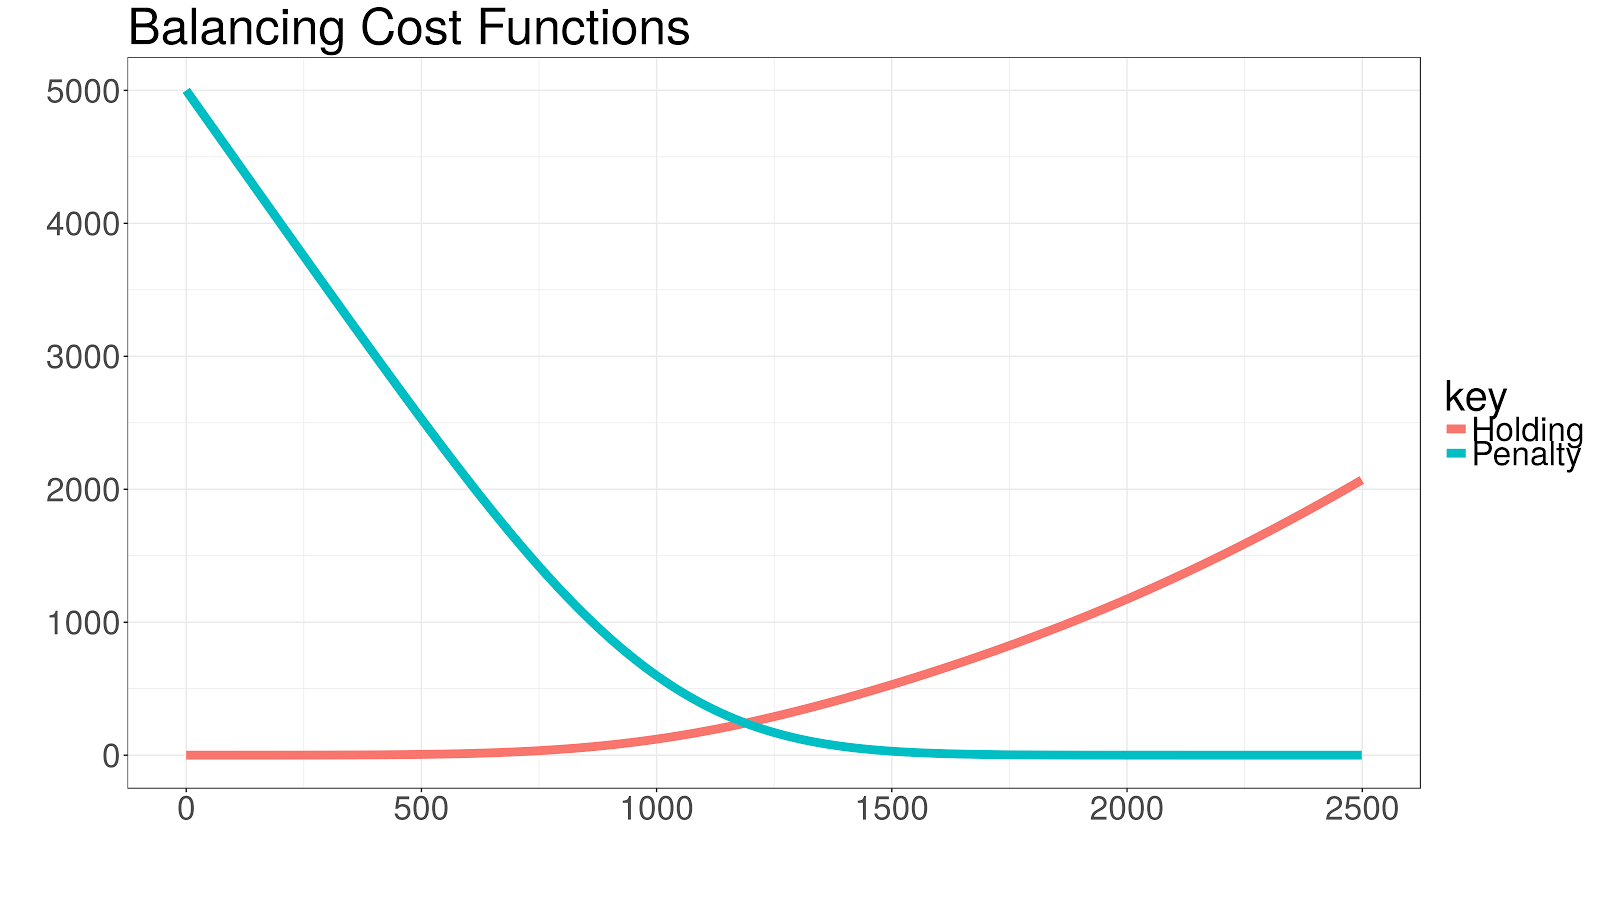
\includegraphics[width=\textwidth]{cost_function_slides}
\end{figure}
\end{frame}

%------------------------------------------------

\section{Computing Balancing Policies}

%------------------------------------------------

\begin{frame}
\frametitle{Computing the Balancing Point}
Newton-Raphson begins with an initial estimate $x_0$, and then iterates the following equation:
$$
	x_{n+1} = x_n + \frac{f(x_n)}{f^{\prime}(x_n)}
$$
For the dual balancing policy, $f$ and $f^{\prime}$ would be defined as follows:
$$
	f(x) = l_s^B(x) - \pi_s^B(x) 
$$
$$
	f^{\prime}(x) =  \frac{d}{dx} l_s^B(x) - \frac{d}{dx} \pi_s^B(x) 
$$
Requires good starting point, $x_0 = \mu$ works well. 
\end{frame}

%------------------------------------------------

\begin{frame}
\begin{figure}
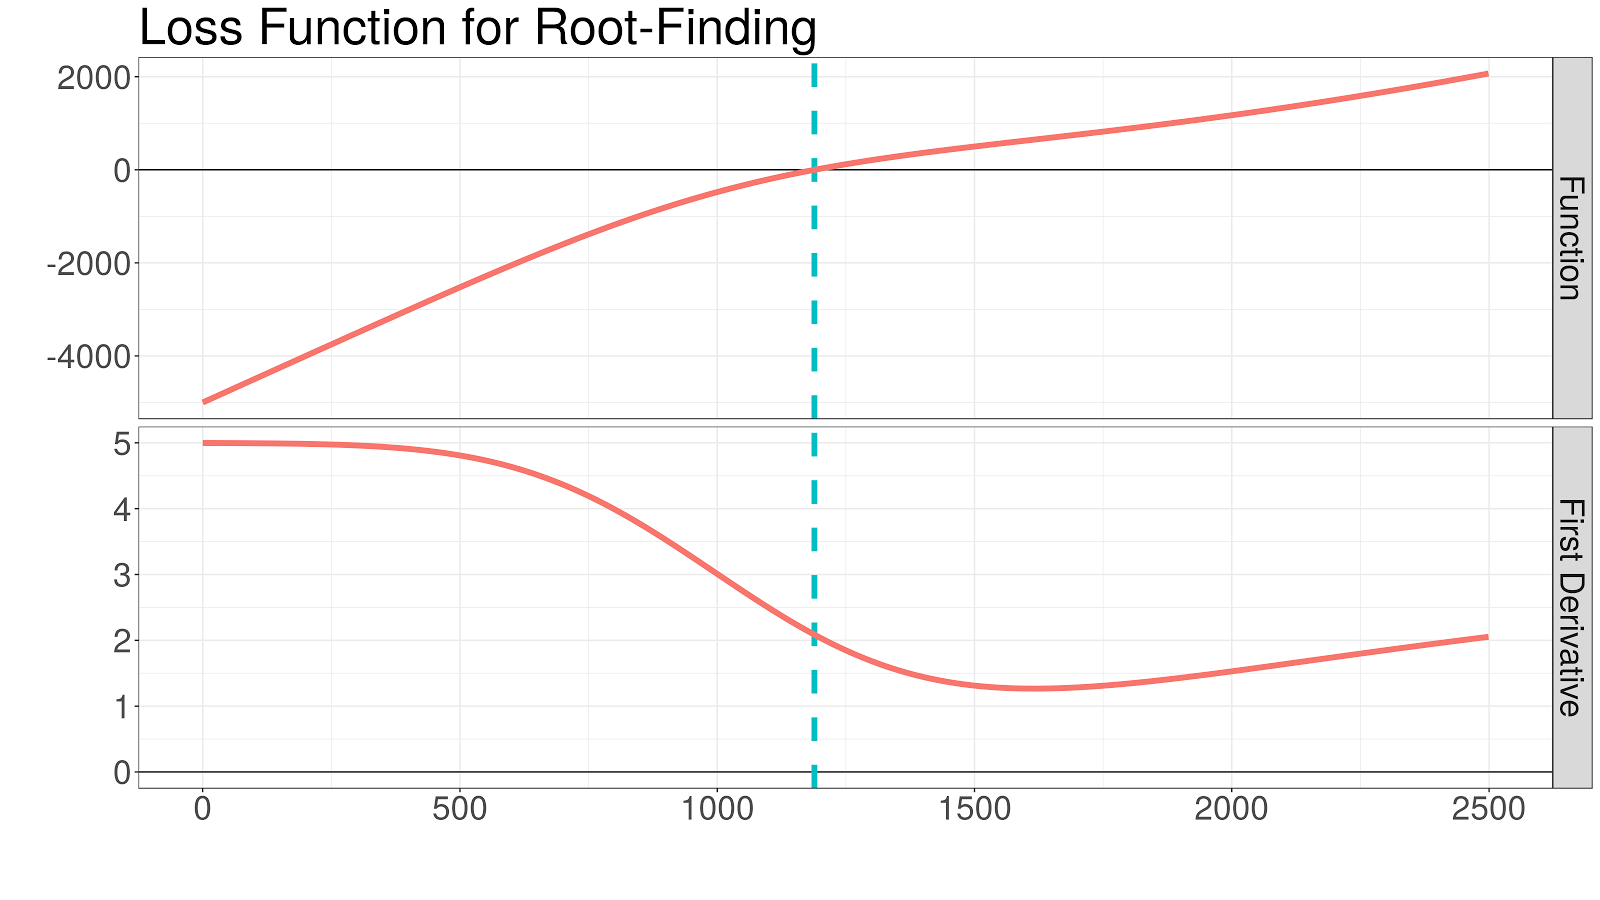
\includegraphics[width=\textwidth]{root_function_slides}
\end{figure}
\end{frame}

%------------------------------------------------

\begin{frame}[shrink=10]
\frametitle{Efficiently Computing the Balancing Point}
Computing holding costs requires a very large integral:
\begin{alignat*}{1}
	l_s^B(q_s) &= \EX \bigg\{\sum_{j=s}^T H_{[s,j]}^B(\vec{D}) \; | \; f_s \bigg\} \\
		&= \int_{z_s=0}^{\infty} \int_{z_{(s+1)}=0}^{\infty}\dots \int_{z_T=0}^{\infty}\sum_{j=s}^T  H_{[s,j]}^B(\vec{z}) d\Phi(z_s, z_{s+1}, \dots z_T) \\
		&= \sum_{j=s}^T \int_{z_s=0}^{\infty} \int_{z_{(s+1)}=0}^{\infty}\dots \int_{z_j=0}^{\infty} H_{[s,j]}^B(\vec{z}) d\Phi(z_s, z_{s+1}, \dots z_j)
\end{alignat*}

Let $\psi_{[s,j]}$ be the cumulative demand distribution. 

\begin{equation*}
	l_s^B(q_s) = \sum_{j=s}^T  h_j \int_{z_j=X_s}^{X_s + q_s}\bigg(q_s + X_s - z_j \bigg) \psi_{[s,j]} (z_j) dz_j
\end{equation*}
For nonincreasing $h_j$, the series in $l_s^B(q_s)$ is nonincreasing with $j$, so series can be truncated.
\end{frame}

%------------------------------------------------

\begin{frame}
\begin{figure}
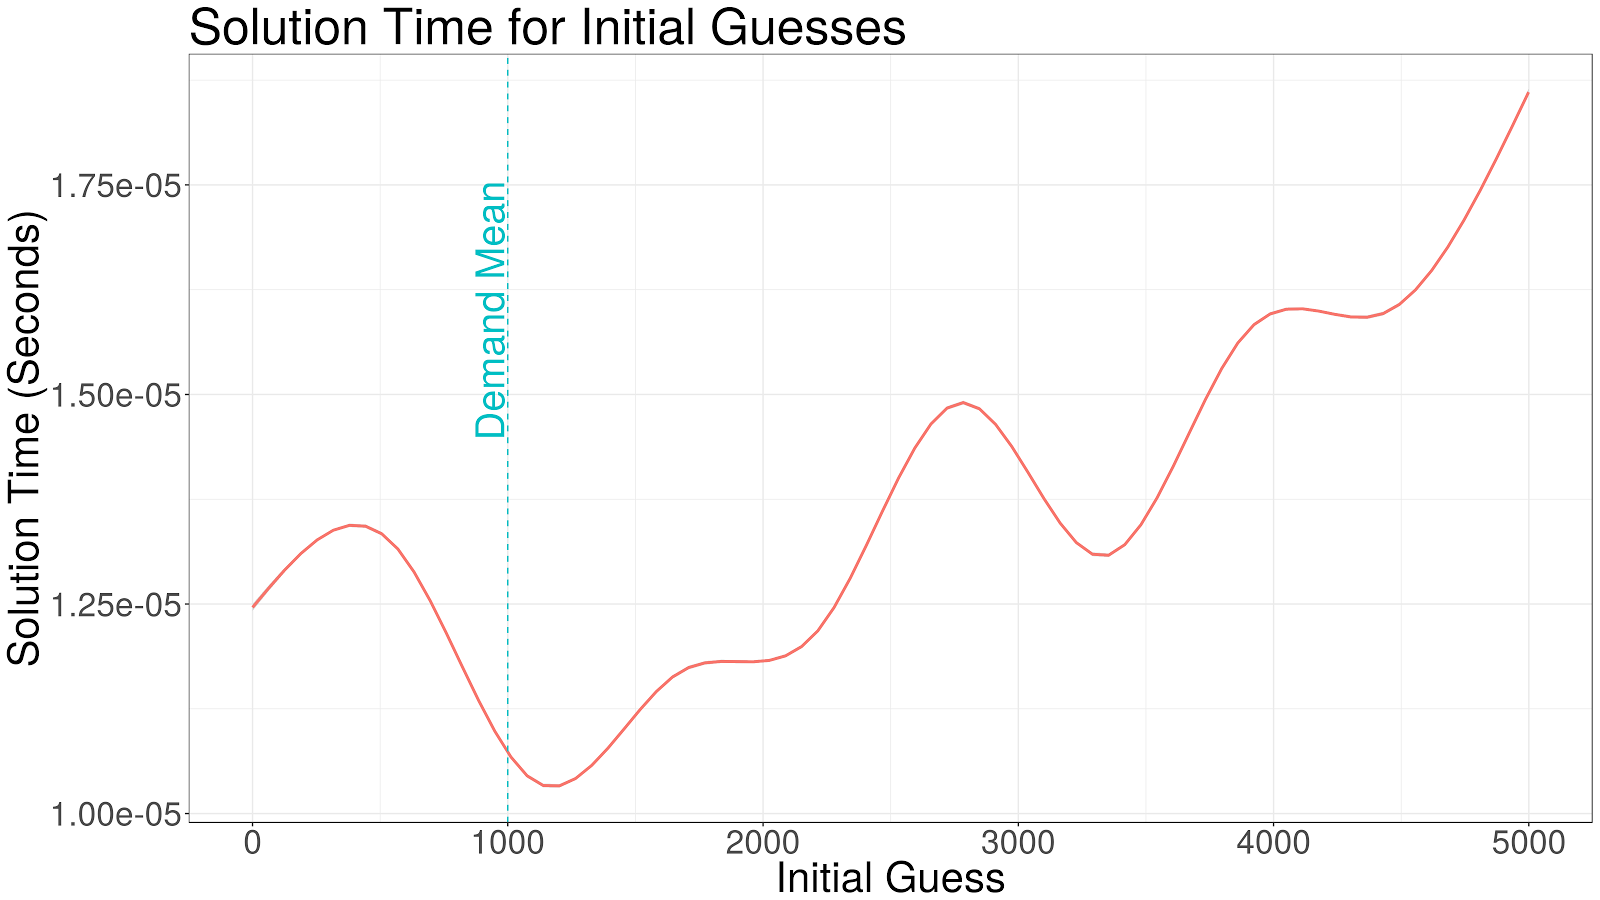
\includegraphics[width=\textwidth]{solution_times_slides}
\end{figure}
\end{frame}

%------------------------------------------------

\begin{frame}
\bibliography{citations}
\bibliographystyle{plainnat}
\end{frame}

%----------------------------------------------------------------------------------------

\end{document} 